\let\negmedspace\undefined
\let\negthickspace\undefined
\documentclass[journal]{IEEEtran}
\usepackage[a5paper, margin=10mm, onecolumn]{geometry}
%\usepackage{lmodern} % Ensure lmodern is loaded for pdflatex
\usepackage{tfrupee} % Include tfrupee package

\setlength{\headheight}{1cm} % Set the height of the header box
\setlength{\headsep}{0mm}     % Set the distance between the header box and the top of the text

\usepackage{gvv-book}
\usepackage{gvv}
\usepackage{cite}
\usepackage{amsmath,amssymb,amsfonts,amsthm}
\usepackage{algorithmic}
\usepackage{graphicx}
\usepackage{textcomp}
\usepackage{xcolor}
\usepackage{txfonts}
\usepackage{listings}
\usepackage{enumitem}
\usepackage{mathtools}
\usepackage{gensymb}
\usepackage{comment}
\usepackage[breaklinks=true]{hyperref}
\usepackage{tkz-euclide} 
\usepackage{listings}
% \usepackage{gvv}                                        
\def\inputGnumericTable{}                                 
\usepackage[latin1]{inputenc}                                
\usepackage{color}                                            
\usepackage{array}                                            
\usepackage{longtable}                                       
\usepackage{calc}                                             
\usepackage{multirow}                                         
\usepackage{hhline}                                           
\usepackage{ifthen}                                           
\usepackage{lscape}
\begin{document}

\bibliographystyle{IEEEtran}
\vspace{3cm}

\title{1.5.34}
\author{EE24BTECH11037 - Manognya Kundarapu
}
% \maketitle
% \newpage
% \bigskip
{\let\newpage\relax\maketitle}

\renewcommand{\thefigure}{\theenumi}
\renewcommand{\thetable}{\theenumi}
\setlength{\intextsep}{10pt} % Space between text and floats


\numberwithin{equation}{enumi}
\numberwithin{figure}{enumi}
\renewcommand{\thetable}{\theenumi}


\textbf{Question}:\\
The point $\vec P$ which divides the line segment joining the points $\vec A\brak{2,-5}$ and $\vec B\brak{5,2}$ in the ratio $2 \colon 3$ lies in which quadrant$?$
\\
\solution
\begin{table}[ht!]    
  \centering
  \begin{tabular}[12pt]{ |c| c|}
    \hline
    \textbf{Variable} & \textbf{Description}\\ 
    \hline
    $\vec P$ & Point dividing $A$ and $B$ in the given ratio \\
    \hline 
    $\vec A$ & point whose coordinates are $\brak{2,-5}$\\
    \hline
    $\vec B$ & point whose coordinates are $\brak{5,2}$\\
    \hline   
    \end{tabular}

  \caption{Variables Used}
  \label{tab10.5.3.9.1}
\end{table}
\begin{align}
\vec P=\frac{A+kB}{k+1}, k=\frac{2}{3}\\
    =\frac{1}{k+1}\brak{A}+\frac{k}{k+1}\brak{B}\\
    =% Parentheses
\begin{pmatrix}
A & B \\
\end{pmatrix}
    % Parentheses
\begin{pmatrix}
\frac{1}{k+1} \\
\frac{k}{k+1}\\
\end{pmatrix}\\
    =% Parentheses
\begin{pmatrix}
2 & 5\\
-5 & 2\\
\end{pmatrix}
% Parentheses
\begin{pmatrix}
\frac{3}{5}\\
\frac{2}{5}\\
\end{pmatrix}
=% Parentheses
\begin{pmatrix}
\frac{16}{5}\\
\frac{-11}{5}\\
\end{pmatrix}
\end{align}
$\therefore$ $\vec P\brak{3.2, -2.2}$. \\ 
$\vec P$ is in \textbf{fourth quadrant}.
\begin{figure}[h!]
   \centering
   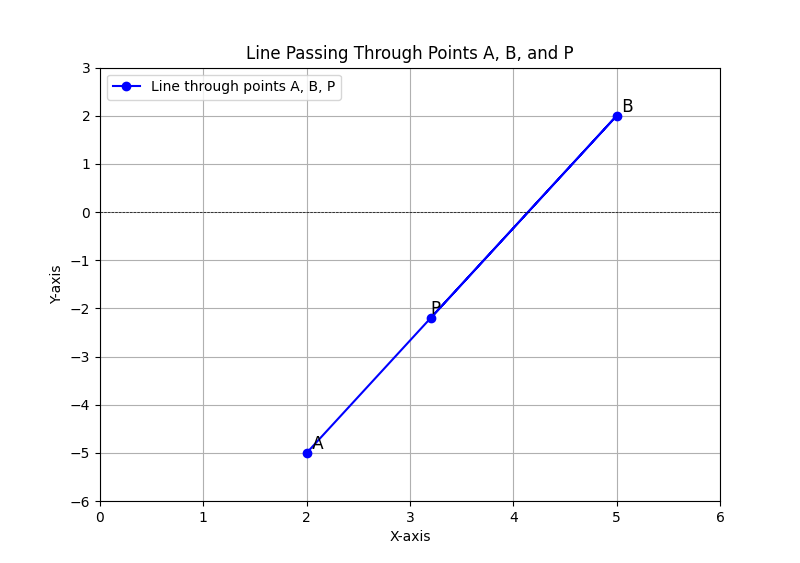
\includegraphics[width=0.7\linewidth]{Figure_1.png}
   \caption{Stem Plot of y\brak{n}}
   \label{stemplot}
\end{figure}
\end{document}  



